%\documentclass{report}
\documentclass[11pt,a4paper,twoside,openright]{book}
\usepackage{geometry}
\geometry{
    a4paper,
    left=30mm,top=20mm,right=25mm,bottom=15mm,
    headheight=12pt,headsep=11mm,foot=0pt,footskip=11mm,
    includeheadfoot
}
\usepackage[utf8]{inputenc}
\usepackage[T1]{fontenc}
\usepackage{graphicx}
\usepackage{chngcntr}
\usepackage{multirow}
\usepackage{longtable}
\usepackage{bbding}
\usepackage{amsmath}
\usepackage{hhline}
\usepackage[a-1a]{pdfx}
\usepackage{hyperref}
\usepackage{mathtools}
\usepackage{booktabs}
\counterwithout{footnote}{chapter}
\setcounter{chapter}{4}


\begin{document}



\chapter{Jets faking photons}

The jets faking photons background represents approximately the 8\% of the total background of the Mono-Photon analysis and it is due to Z + jet or W + jet events in which the jet is mistakenly reconstructed and identified as a photon. The classification of the reconstructed object into a photon or a jet is performed by an algorithm based on the detector inputs. This algorithm necessarily introduces an efficiency for true photons and a jet contamination in a selected sample of photons. The simulations do not describe accurately the performance of this algorithm, so the jet $\rightarrow$ $\gamma$ fraction is estimated with a purely data-driven technique. This is done applying the \textit{Two Dimensional Sideband Method}, which was used in 2015 and 2016 analysis too.
In this chapter the method, the validation and the results of the estimation of the jets faking photons background in all the regions of the 2019 ATLAS' Mono-Photon analysis using the full 2015-2018 Run 2 statistics will be presented.


\section{Basic method}

The \textit{Two Dimensional Sideband Method}, also known as the ABCD method, is an almost data-driven technique employed to determine a background contamination in a given signal region. This method relies on counting photon candidates in four regions of a two-dimensional plane defined by an isolation variable and an identification variable (tightness). The identification variable is represented by the value of $TopoEtCone40 - 0.022p_{T} - 2.45$ GeV, described in Sec. \ref{Isolation}: the candidate photon is considered isolated if it is lower than 0 GeV, not-isolated if it is greater than 3 GeV. Note that the gap of 3 GeV is defined to minimize signal leakage in the CRs. On the other hand the identification variable is divided in two bins corresponding to the Tight and Tight-4 selections described in Sec. \ref{Identification}. Tight-3 and Tight-5 selections will be used to estimate systematic uncertainties. 

The plane is so divided into four regions as shown in Fig. \ref{fig:ABCD}, where the signal region corresponds to the Tight-Isolated region and the three CRs are assumed to be populated only by background photons. In each region the number of candidate photons is:

\begin{itemize}
    
    \item[-] $N^{A}$: number of Tight - Isolated candidates;
    \item[-] $N^{B}$: number of Tight - Not-isolated candidates;
    \item[-] $M^{A}$: number of Tight-4 - Isolated candidates;
    \item[-] $M^{B}$: number of Tight-4 - Not-isolated candidates.

\end{itemize}


\begin{figure}[hbtp!]
    \centering
    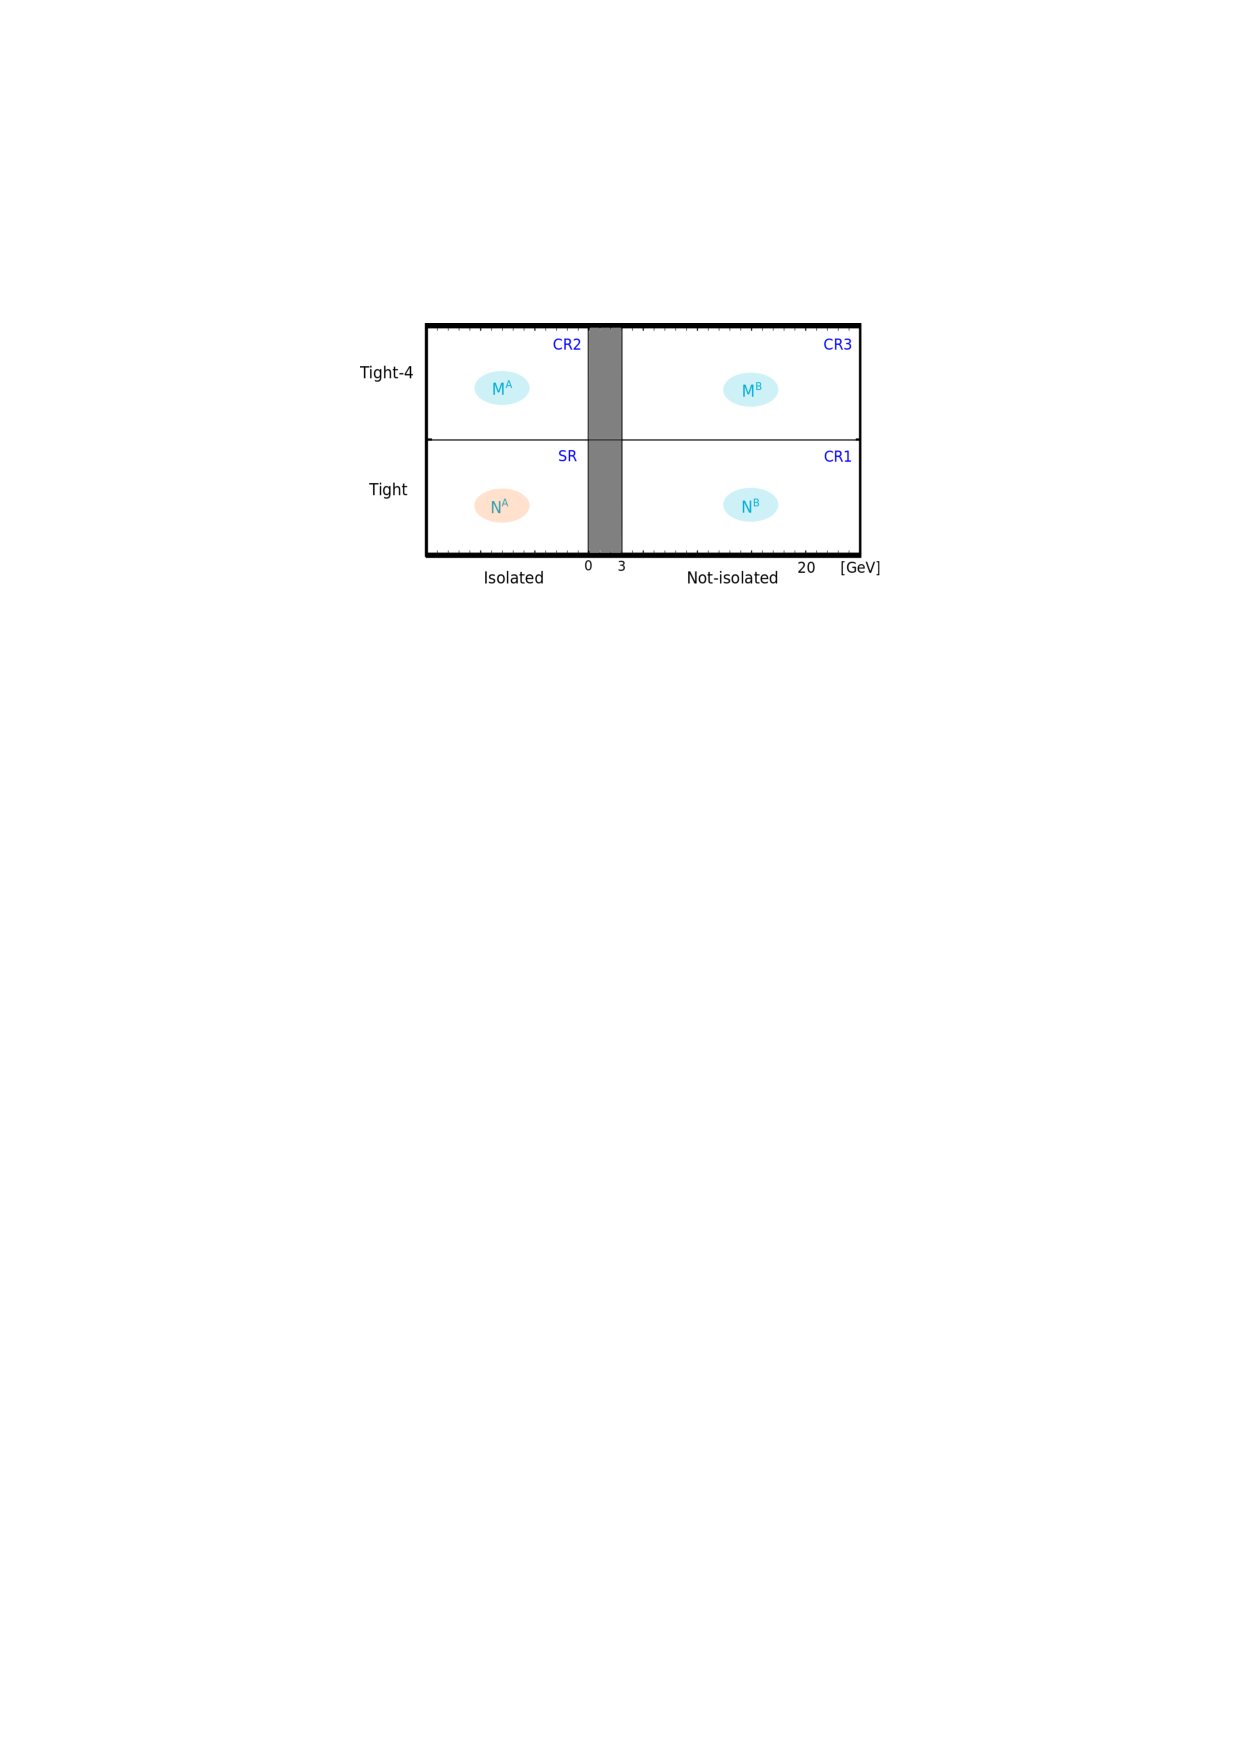
\includegraphics[width=10cm]{ABCD.pdf}
    \caption{Scheme of the regions defined by the Two Dimensional Sideband Method.}
    \label{fig:ABCD}
\end{figure}

For real data the numbers of signal and background photon candidates in the SR are defined as $N^{A}_{sig}$ and $N^{A}_{bkg}$ respectively, while for MC simulation as $N^{A}_{sigMC}$ and $N^{A}_{bkgMC}$ (and similarly in the CRs).

The method relies on two simplifying hypotheses:

\begin{enumerate}

    \item the correlation between tightness and isolation is negligible for the background;
    
    \item in the three CRs the number of signal photon candidates is negligible compared to the number of fake candidates:
    
    \begin{equation}
    \begin{aligned}
        N^{B}_{bkg} & \gg N^{B}_{sig}\\
        M^{A}_{bkg} & \gg M^{A}_{sig}\\
        M^{B}_{bkg} & \gg M^{B}_{sig}
    \end{aligned}
    \end{equation}
    
    
    
\end{enumerate}

The first assumption leads to:

\begin{equation} \label{eq:correlation_factor_1}
    \frac{N^{A}_{bkg}}{N^{B}_{bkg}} = \frac{M^{A}_{bkg}}{M^{B}_{bkg}}
\end{equation}



while the second one implies that:

\begin{equation}
\begin{aligned}
    N^{B} & = N^{B}_{bkg}\\
    M^{A} & = M^{A}_{bkg}\\
    M^{B} & = M^{B}_{bkg}
\end{aligned}
\end{equation}

Therefore, combining the two hypotheses:

\begin{equation}
    N^{A}_{bkg} = N^{B} \frac{M^{A}}{M^{B}}
\end{equation}

that leads directly to:

\begin{equation} \label{eq:Nasig}
    N^{A}_{sig} = N^{A} - N^{A}_{bkg} = N^{A} - N^{B} \frac{M^{A}}{M^{B}}
\end{equation}

\begin{equation}
    P \coloneqq \frac{N^{A}_{sig}}{N^{A}} = 1 - \frac{N^{B}}{N^{A}} \frac{M^{A}}{M^{B}}
\end{equation}{}

where the purity $P$ of the sample is defined as the ratio of the number of signal photons and the total number of candidates in the SR.

A purely data-driven formula for the purity is then obtained even if it requires that both the two hypotheses are satisfied, although this is not always the case.


\subsection{Correlation in the background}

By means of MC simulations it is possible to take into account non-negligible correlations in the background 2D distributions. Assuming that MC and real data are in good agreement for background events, the number of candidates in a given region can be approximated with the corresponding MC prediction. This is done in the following way:

\begin{equation} \label{eq:eq1}
\begin{aligned}
    N^{A}_{sig} & = N^{A} - N^{A}_{bkg} = N^{A} - N^{A}_{bkg} \frac{N^{B}_{bkg} \times M^{A}_{bkg}/M^{B}_{bkg}}{N^{B}_{bkg} \times M^{A}_{bkg}/M^{B}_{bkg}} \\
    & = N^{A} - \biggl( N^{B}_{bkg} \frac{M^{A}_{bkg}}{M^{B}_{bkg}} \biggr) \biggl( \frac{N^{A}_{bkg}}{N^{B}_{bkg}} \frac{M^{B}_{bkg}}{M^{A}_{bkg}} \biggr) \\
    & \approx N^{A} - \biggl( N^{B}_{bkg} \frac{M^{A}_{bkg}}{M^{B}_{bkg}} \biggr) \biggl( \frac{N^{A}_{bkgMC}}{N^{B}_{bkgMC}} \frac{M^{B}_{bkgMC}}{M^{A}_{bkgMC}} \biggr) \\
    & \approx N^{A} - \biggl( N^{B} \frac{M^{A}}{M^{B}} \biggr) \biggl( \frac{N^{A}_{bkgMC}}{N^{B}_{bkgMC}} \frac{M^{B}_{bkgMC}}{M^{A}_{bkgMC}} \biggr) \\
    & = N^{A} - \biggl( N^{B} \frac{M^{A}}{M^{B}} \biggr) R_{MC}
\end{aligned}
\end{equation} 

that implicitly defines the \textit{correlation factor} $R_{MC}$ which can be estimated by means of pure background MC simulations. Its statistical uncertainty is obtained by the error propagation:

\begin{equation}
    \sigma_{R_{MC}} = R_{MC} \sqrt{\frac{1}{N^{A}_{bkgMC}} + \frac{1}{N^{B}_{bkgMC}} + \frac{1}{M^{A}_{bkgMC}} + \frac{1}{M^{B}_{bkgMC}}}
\end{equation}

which depends only on the available MC statistic.

\subsection{Signal leakage}

MC simulations can also estimate the signal leakage from the SR to each one of the CRs, releasing thus the second hypothesis. As for the correlation factor, real photons are approximated with MC simulations, assuming non negligible signal contamination in the CRs, the number of events in these regions can be written as:

\begin{equation}
\begin{aligned}
    N^{B} & = N^{B}_{bkg} + N^{B}_{sig} = N^{B}_{bkg} + N^{A}_{sig} \frac{N^{B}_{sig}}{N^{A}_{sig}} \\
    M^{A} & = M^{A}_{bkg} + M^{A}_{sig} = M^{A}_{bkg} + N^{A}_{sig} \frac{M^{A}_{sig}}{N^{A}_{sig}} \\
    M^{B} & = M^{B}_{bkg} + M^{B}_{sig} = M^{B}_{bkg} + N^{A}_{sig} \frac{M^{B}_{sig}}{N^{A}_{sig}} 
\end{aligned}
\end{equation}

\clearpage
Three \textit{signal leakage coefficients} are then defined as:

\begin{equation}
\begin{aligned}
    \frac{N^{B}_{sig}}{N^{A}_{sig}} & \coloneqq c_{1} \approx \frac{N^{B}_{sigMC}}{N^{A}_{sigMC}} \\
    \frac{M^{A}_{sig}}{N^{A}_{sig}} & \coloneqq c_{2} \approx \frac{M^{A}_{sigMC}}{N^{A}_{sigMC}} \\
    \frac{M^{B}_{sig}}{N^{A}_{sig}} & \coloneqq c_{3} \approx \frac{M^{B}_{sigMC}}{N^{A}_{sigMC}} \\
\end{aligned}
\end{equation}

A schematic representation of the meaning of signal leakage coefficients is reported in Fig. \ref{fig:Signal_Leakage}.

\begin{figure}
    \centering
    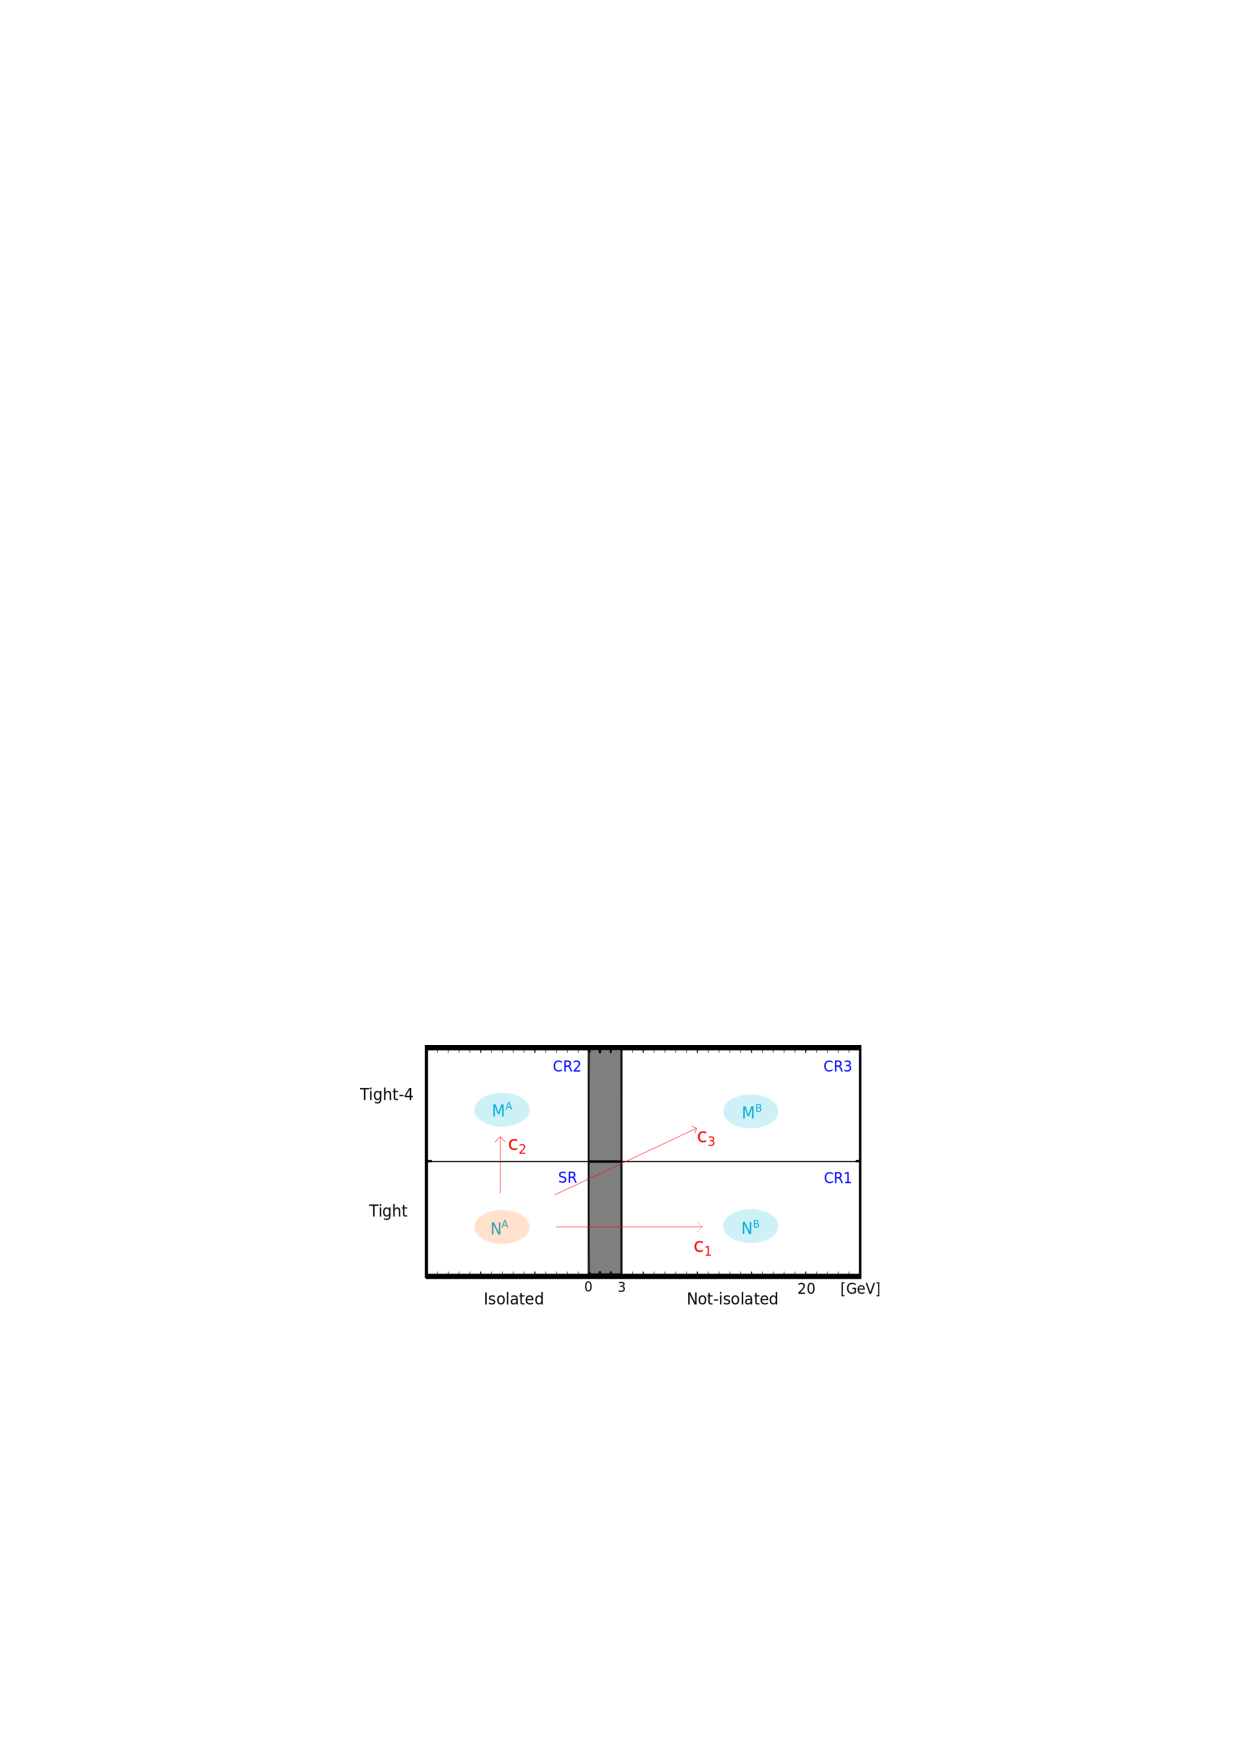
\includegraphics[width=10cm]{Signal_Leakage.pdf}
    \caption{Representation of the signal leakage coefficients.}
    \label{fig:Signal_Leakage}
\end{figure}

Applying these coefficients to Eq. \ref{eq:Nasig} leads to:

\begin{equation}
    N^{A}_{sig} = N^{A} - N^{B}_{bkg} \frac{M^{A}_{bkg}}{M^{B}_{bkg}} = N^{A} - (N^{B} - N^{A}_{sig} c_{1}) \frac{M^{A} - N^{A}_{sig} c_{2}}{M^{B} - N^{A}_{sig} c_{3}}
\end{equation}

and resolving for $N^{A}_{sig}$ gives the number of signal photons in the SR corrected for signal leakage in the CRs:

\begin{equation}
    N^{A}_{sig} = \frac{\bigl(M^{B} + N^{A}c_{3} - N^{B}c_{2} - M^{A}c_{1}\bigr)\bigl(-1 + \sqrt{1 + \frac{4(c_{1}c_{2} - c_{3})(N^{A}M^{B} - N^{B}M^{A})}{(M^{B} + N^{A}c_{3} - N^{B}c_{2} - M^{A}c_{1})^{2}}}\bigr)}{2(c_{1}c_{2} - c_{3})}
\end{equation}


\subsection{Signal yields and purity} \label{Purity}

It is now possible to account for both signal leakage and correlation in the background at the same time. Starting from Eq. \ref{eq:eq1}:

\begin{equation}
    N^{A}_{sig} \approx N^{A} - \biggl( N^{B}_{bkg} \frac{M^{A}_{bkg}}{M^{B}_{bkg}} \biggr) \biggl( \frac{N^{A}_{bkgMC}}{N^{B}_{bkgMC}} \frac{M^{B}_{bkgMC}}{M^{A}_{bkgMC}} \biggr)
\end{equation}

replacing $N^{B}_{bkg}$ with $N^{B} - N^{A}_{sig}c_{1}$ and so on:

\begin{equation}
    N^{A}_{sig} \approx N^{A} - \biggl( (N^{B} - N^{A}_{sig} c_{1}) \frac{M^{A} - N^{A}_{sig} c_{2}}{M^{B} - N^{A}_{sig} c_{3}} \biggr) R_{MC}
\end{equation}

some simple algebra gives $N^{A}_{sig}$ and dividing by $N^{A}$ one finds a formula for the purity which accounts for both corrections:

\begin{equation} \label{eq:final_Na_sig}
\begin{aligned}
    P = &\frac{\bigl(M^{B} + N^{A}c_{3} - N^{B}c_{2}R_{MC} - M^{A}c_{1}R_{MC}\bigr)}{2N^{A}(c_{1}c_{2}R_{MC} - c_{3})} \\
    &\cdot \biggl(-1 + \sqrt{1 + \frac{4(c_{1}c_{2}R_{MC} - c_{3})(N^{A}M^{B} - N^{B}M^{A}R_{MC})}{(M^{B} + N^{A}c_{3} - N^{B}c_{2}R_{MC} - M^{A}c_{1}R_{MC})^{2}}}\biggr)
\end{aligned}
\end{equation} 

The derivatives needed for errors propagation are computed with Mathematica \cite{Mathematica}, a modern technical computing system that enables, among other things, to compute derivatives of an analytical expression of a function.

The systematic uncertainties are estimated varying different assumptions of the method. For example the not-tight control region is moved from Tight-4 to Tight-3 and Tight-5 and two new purities are obtained. The maximum difference between these purities with the nominal one is quoted as systematic uncertainty from the not-tight selection. The same will be done moving the isolation gap from 3 GeV to 2 GeV and 4 GeV, and similarly for the sysematic uncertainties on the four coefficients. The total systematic uncertainty is the square sum of all systematic uncertainties.

\section{Validation test}

To evaluate the consistency of the method, it has been tested on a mixed MC sample of W($\mu \nu$) + $\gamma$ and W + jets events with known purity. The samples are all MC generated with Sherpa \cite{Sherpa} at NLO\footnote{Events are typically weighted by the process cross section. MC samples at NLO (Next to Leading Order) are characterized by weights assigned to each event to properly reproduce the normalization and kinematics of the process.}.

The correlation factor and the signal leakage coefficients have been computed on the mixed sample matching the photon candidates with true-level\footnote{MC simulations are obtained in three steps: at first the particles are generated, then they are simulated to interact with the detector and in the end they are reconstructed with the same procedure used for real data. In this process the generation stage is also known as \textit{true-level}.} jets (for $R_{MC}$) and with true-level photons (for $c_{1}$,$c_{2}$ and $c_{3}$). A particular focus is given to the SR - ISR1 as it is the most populated region.

Results in the SR - ISR1 for the coefficients, with statistical uncertainties, are reported in Table \ref{tab:validation_coeff}:

\begin{table}[!htbp]
    \centering
    \begin{tabular}{cccc}
    \toprule
    $R_{MC}$ & $c_{1}$ & $c_{2}$ & $c_{3}$ \\ \midrule
    2.76 $\pm$ 0.49 & 7.08 $\pm$ 0.80 \% & 4.50 $\pm$ 0.63 \% & 0.49 $\pm$ 0.21 \%\\ \bottomrule
    \end{tabular}
    \caption{Coefficients used in the validation test.}
    \label{tab:validation_coeff}
\end{table}{}


The results for the purities with propagated and systematic uncertainties respectively are reported in Table \ref{tab:validation_purities}:

\begin{table}[!htbp]
    \centering
    \begin{tabular}{cc}
    \toprule
     & Purity \\ \midrule
    True & 84.27 \%\\ \midrule
    Calculated & 86.41 $\pm$ 5.87 $\pm$ 7.26 \%\\ \bottomrule
    \end{tabular}
    \caption{Table of purities calculated to validate the ABCD method.}
    \label{tab:validation_purities}
\end{table}{}

As can be noticed the calculated purities are compatible within the errors with the expected results.


\section{Coefficients from MC}

Once validated the method on a simplified MC sample it is possible to start analyzing different MCs (all NLO Sherpa samples) to get the coefficients needed by the method and assess the systematic uncertainties.


At first very strange results have been observed due to large negative weights, in few events especially in the CRs of the Mono-Photon analysis. These anomalous weights led to very high unnatural correlation factors.

This difficulty has been managed in the following way:

\begin{itemize}

    \item weights with an absolute value > 100 are rescaled to 1;
    
    \item events with $p_{T} < 140$ GeV at truth-level are excluded: the analysis selects candidate photons with $p_{T} > 150$ GeV, but some events can be reconstructed with higher $p_{T}$, with respect to true-level $p_{T}$, possibly gaining a very high cross section weight;

    \item regions where a certain sample (W/Z + $\gamma$/jets) is dominant have been merged to increase statistics:
    \begin{itemize}
    
        \item[-] W + $\gamma$/jets $\rightarrow$ SR + 1muCR;
        
        \item[-] Z + $\gamma$/jets $\rightarrow$ SR + 2muCR + 2eCR;
        
        \item[-] the gammajetCR has been treated separately as it has a different $E_{T}^{miss}$ cut.
        
    \end{itemize}
    
    \item the track isolation ($ptcone20/p_{T}$) has been released in the CRs of the method:
    \begin{itemize}
    
        \item[-] not-isolated events are now those which fail the calorimetric isolation OR the track isolation;
        
        \item[-] a gap of 0.05 on the track isolation variable has been excluded to prevent signal leakage.
    
    \end{itemize}
    
\end{itemize}


Upper limits on track and calorimetric isolation have been set, respectively to 1 and 140 GeV, to exclude pathological events.

\subsection{Signal leakage coefficients}

Signal leakage coefficients have been calculated using three signal samples of Z($ll$) + $\gamma$, Z($\nu \nu$) + $\gamma$ and W + $\gamma$. Results are reported in Fig. \ref{fig:c1}, \ref{fig:c2} and \ref{fig:c3}.


\begin{figure}[hbtp!]
    \centering
    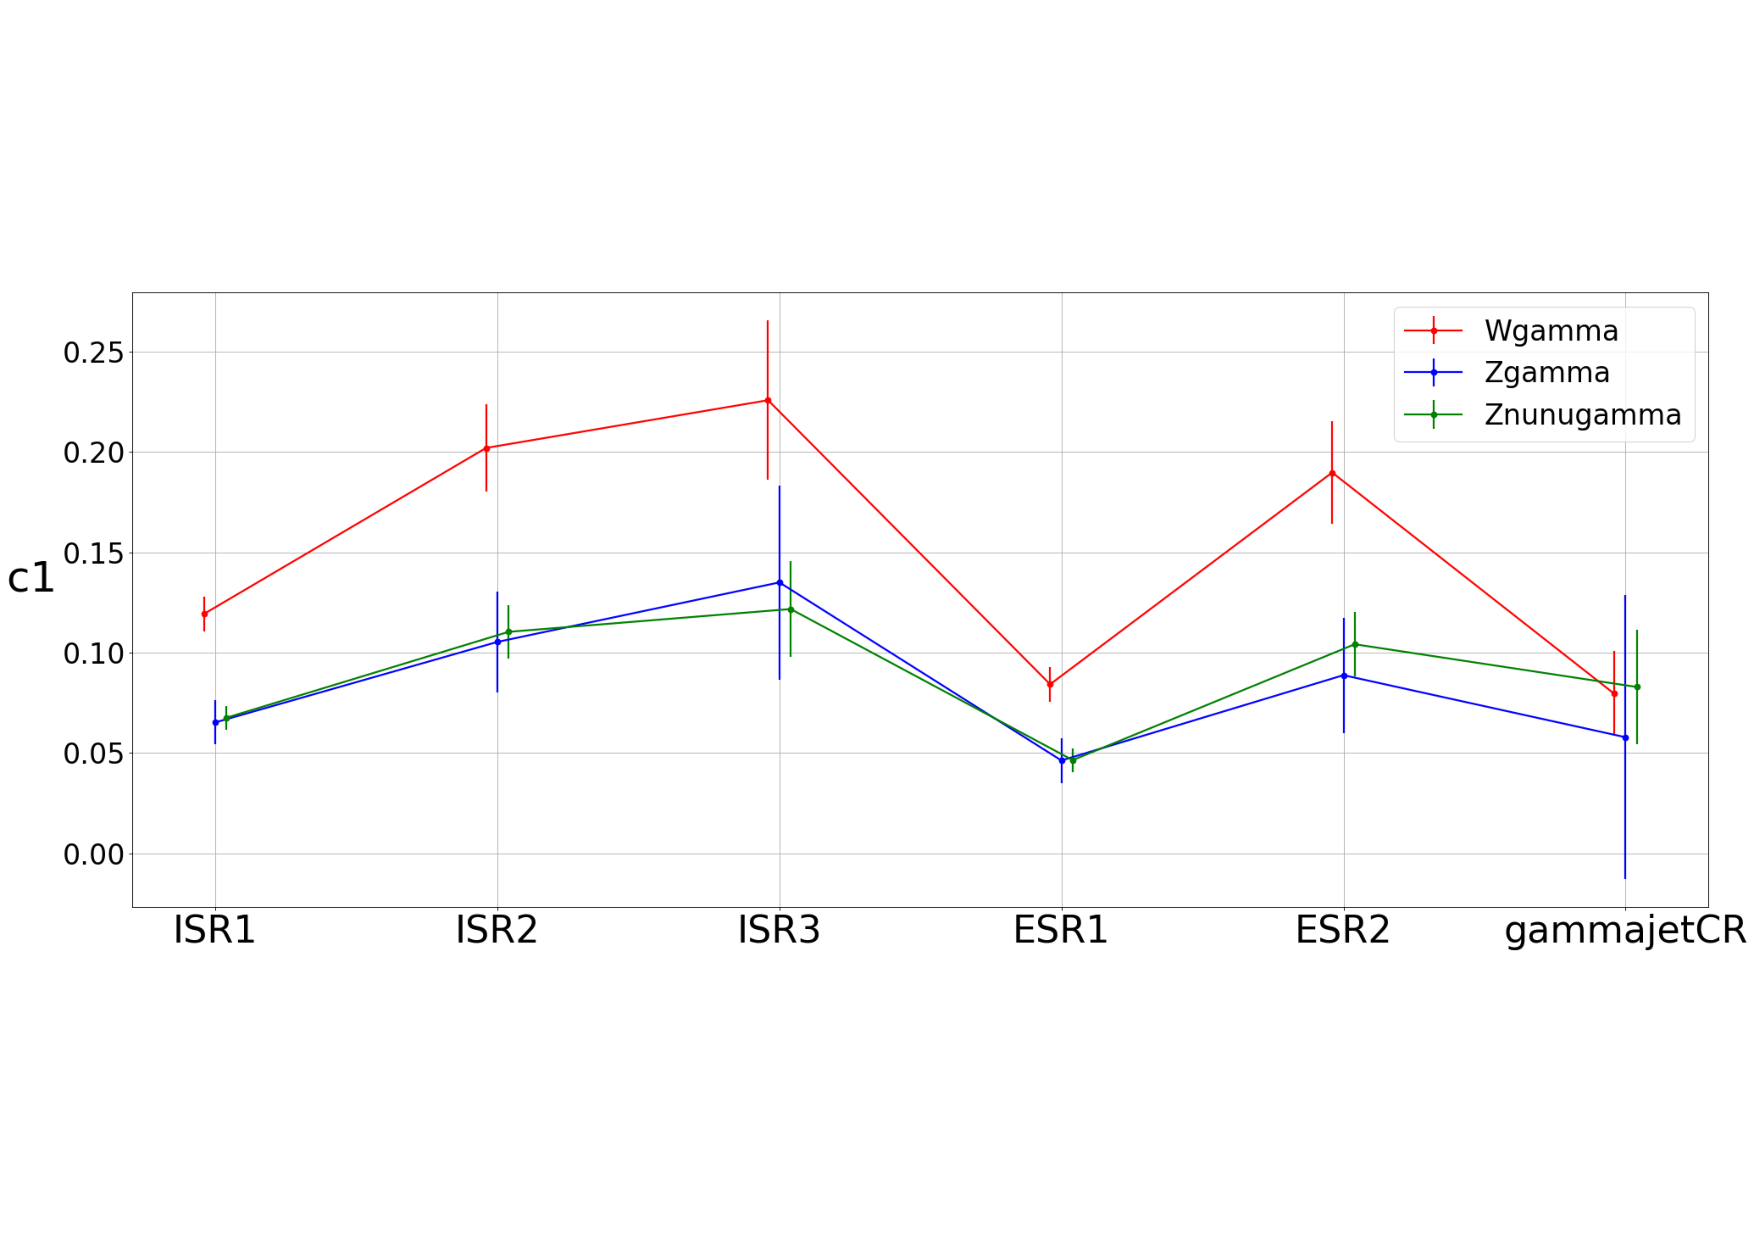
\includegraphics[width=12cm]{c1.pdf}
    \caption{Representation of the signal leakage coefficients $c_{1}$, accounting for signal leakage in the tight - not-isolated region.}
    \label{fig:c1}
\end{figure}


\begin{figure}[hbtp!]
    \centering
    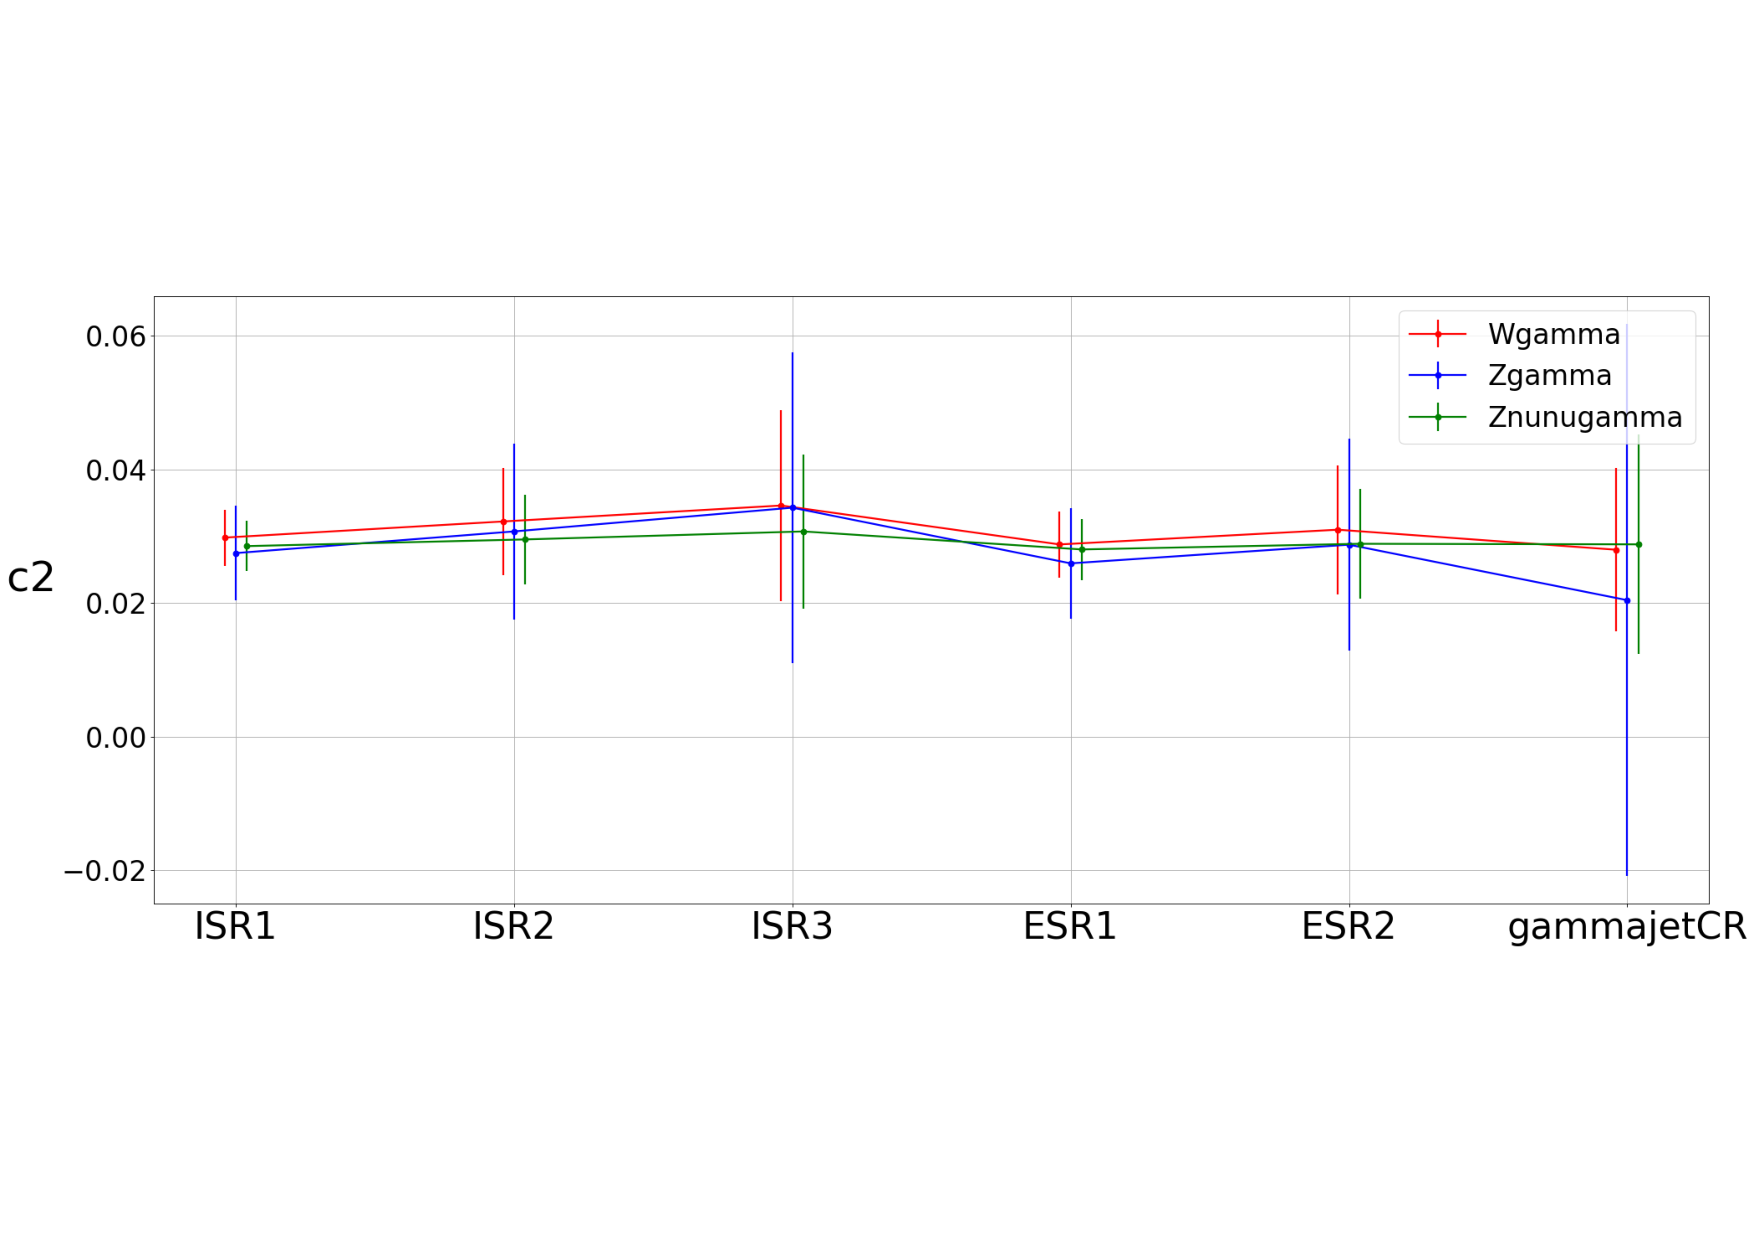
\includegraphics[width=12cm]{c2.pdf}
    \caption{Representation of the signal leakage coefficients $c_{2}$, accounting for signal leakage in the not-tight - isolated region.}
    \label{fig:c2}
\end{figure}

\begin{figure}[hbtp!]
    \centering
    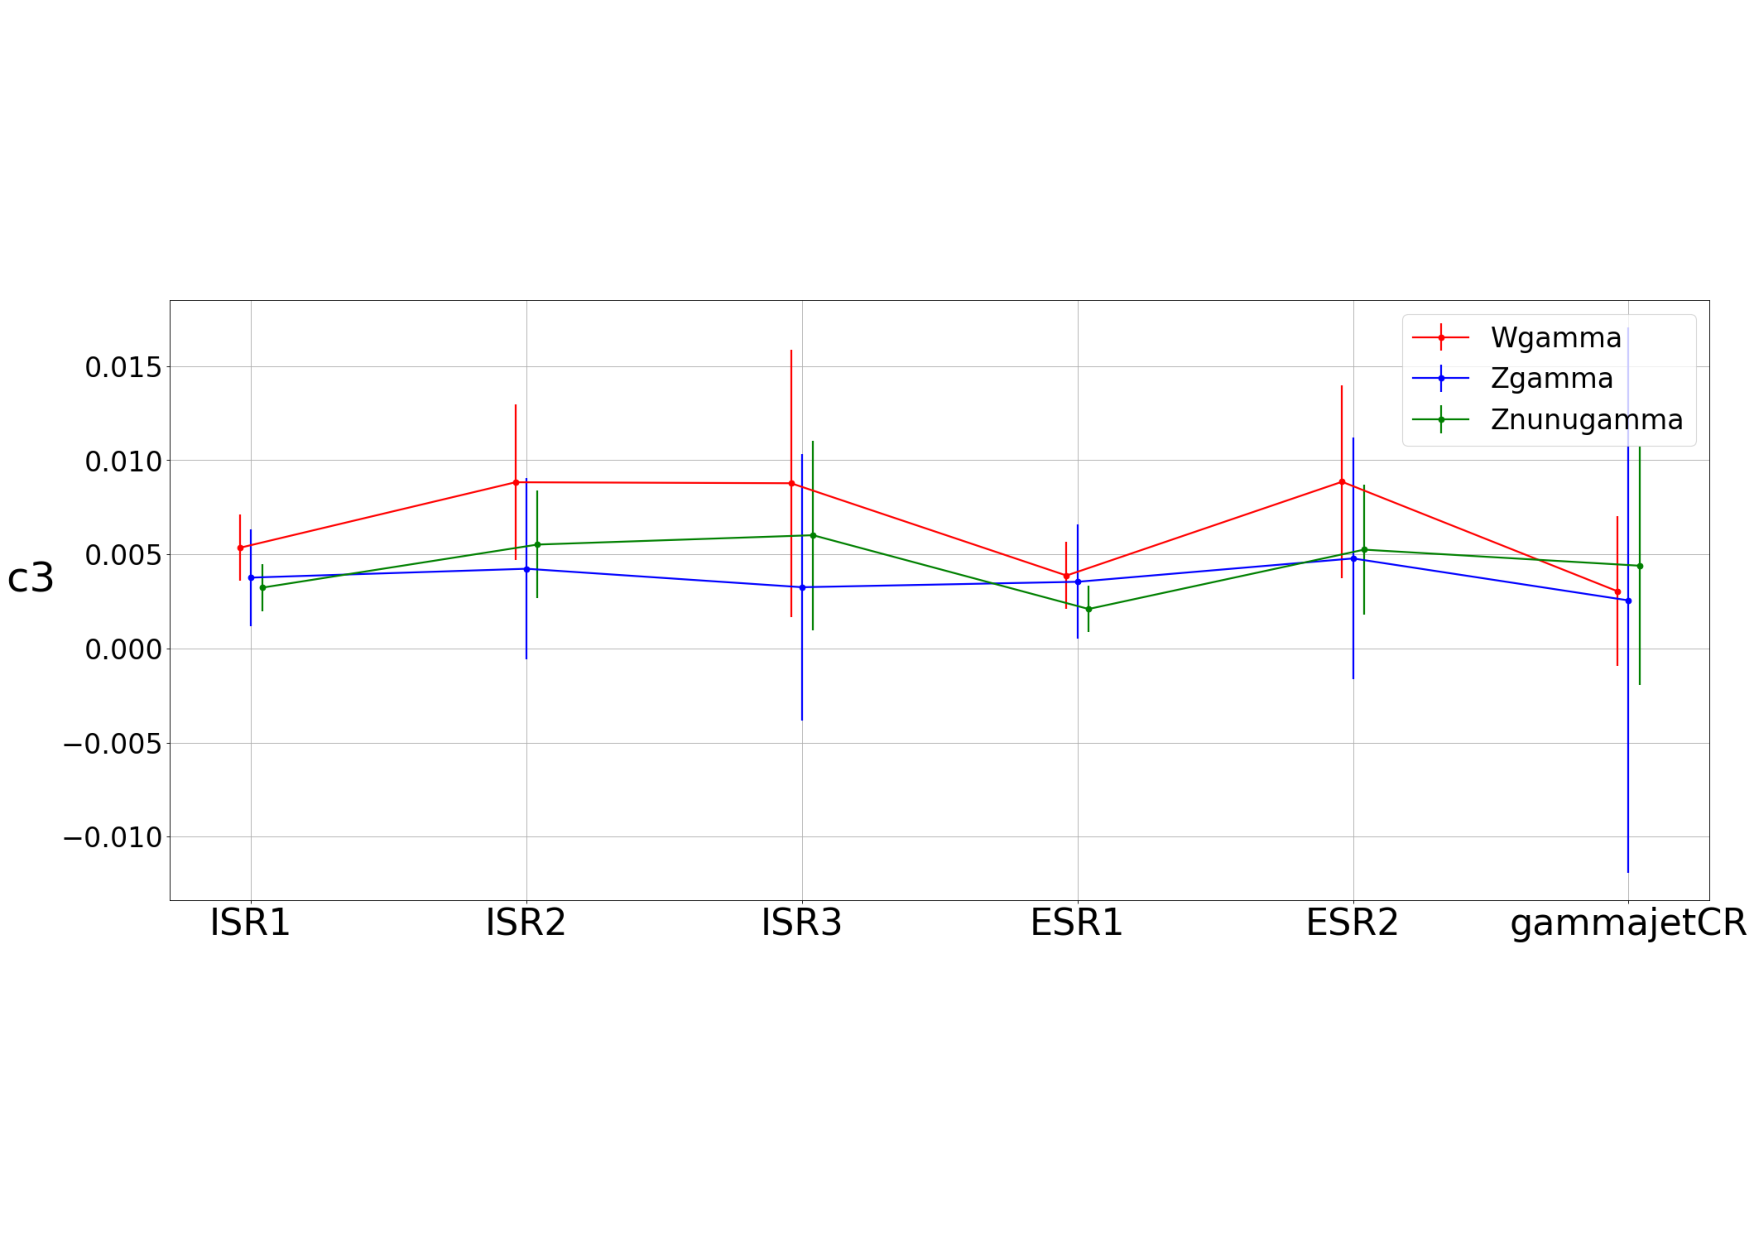
\includegraphics[width=12cm]{c3.pdf}
    \caption{Representation of the signal leakage coefficients $c_{3}$, accounting for signal leakage in the not-tight - not-isolated region.}
    \label{fig:c3}
\end{figure}





\begin{figure}[hbtp!]
    \centering
    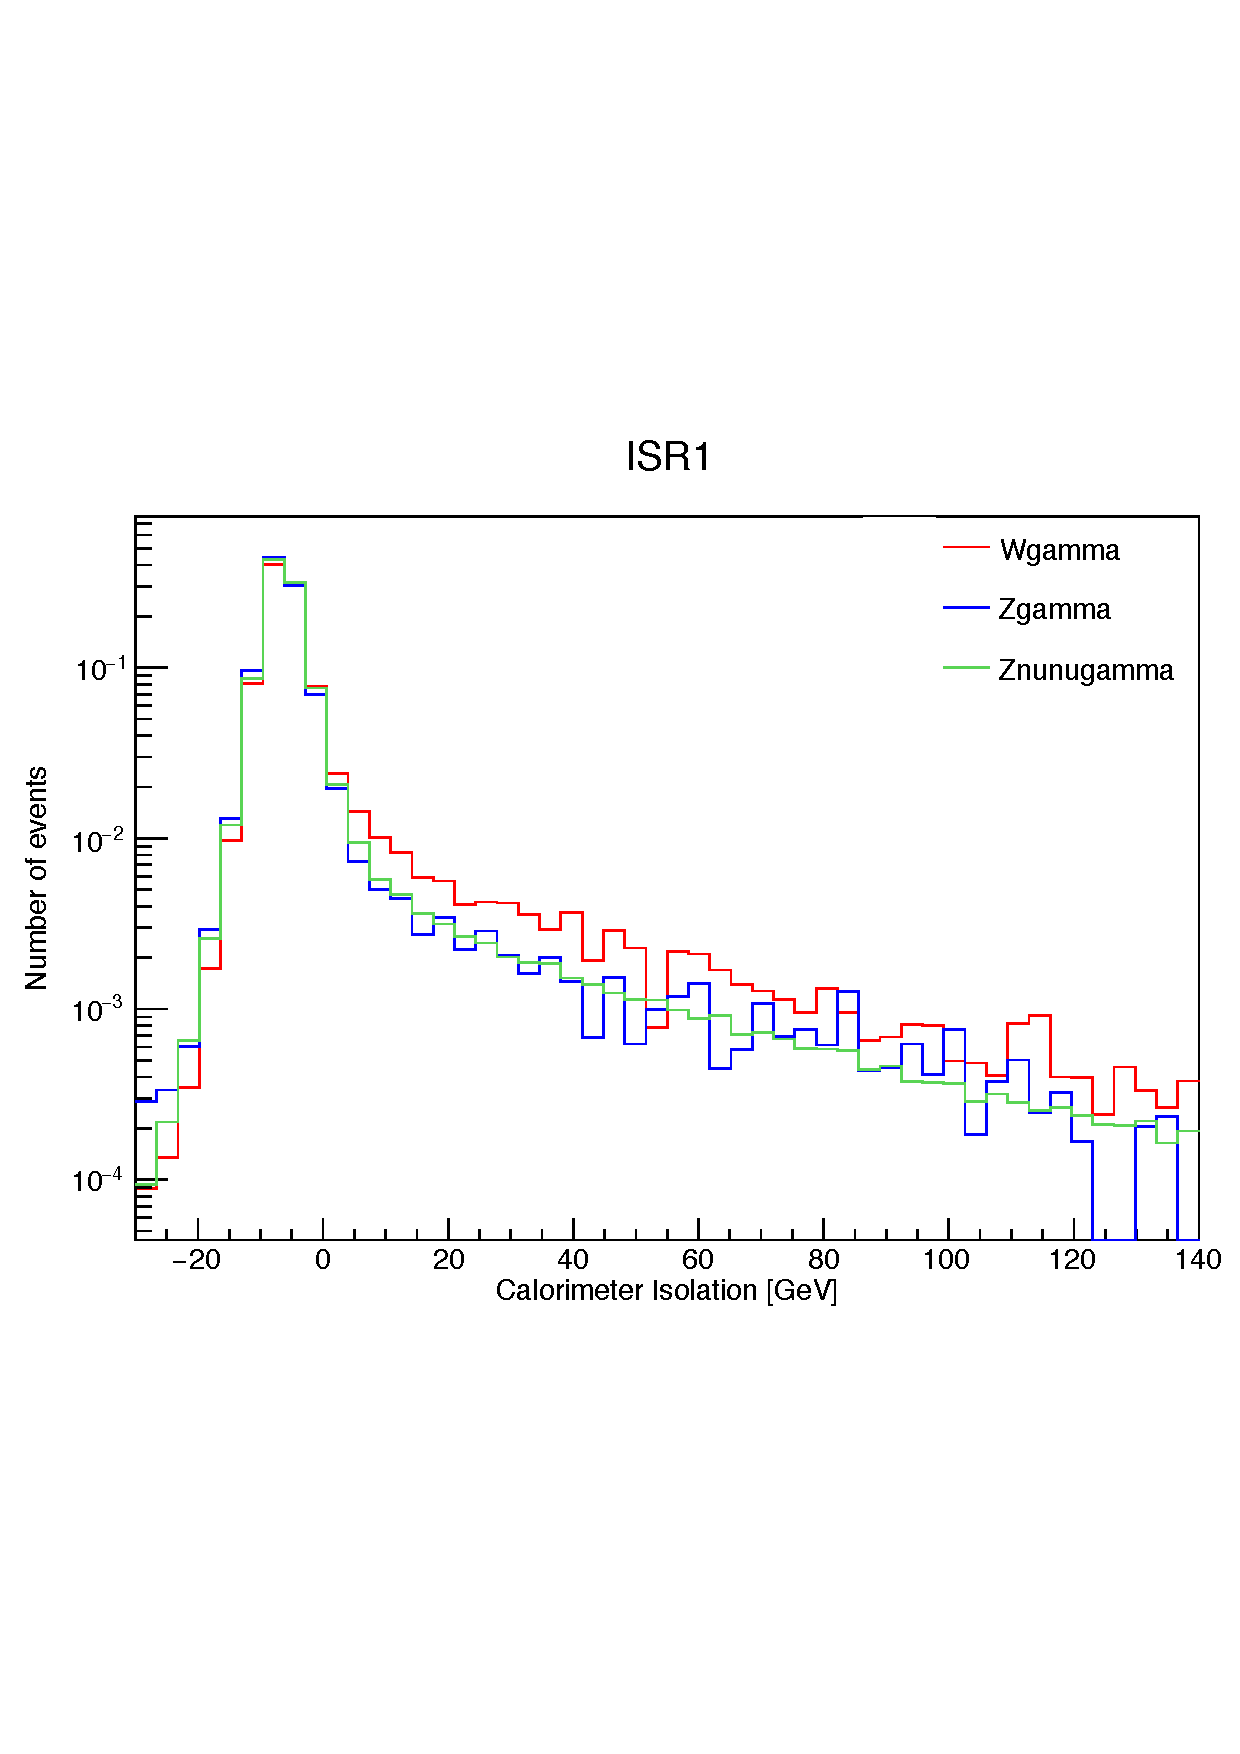
\includegraphics[width=10cm]{c1_isolation_profiles.pdf}
    \caption{Normalized calorimetric isolation profiles in the ISR1 of the three MC samples used to compute the signal leakage coefficients.}
    \label{fig:c1_isolation_profiles}
\end{figure}

A systematic difference between $c_{1}$ coefficients calculated from W and Z bosons samples is evident in the first plot. Fig. \ref{fig:c1_isolation_profiles} shows the normalized calorimetric isolation profiles in the ISR1, where a difference in the tails of the distributions is clearly visible, that results in a systematic difference in the coefficients that accounts for signal leakage from isolated to not-isolated regions. Since the origin of this effect is not fully understood a systematic uncertainty is assigned to $c_{1}$ coefficients to cover the differences observed between different samples. Also $c_{3}$ is thus affected by this systematic, even if the results are compatible.

It can be noticed also a systematic increase of $c_{1}$ and $c_{3}$ with the increase of the $E_{T}^{miss}$ threshold. This behaviour is once again explained by the calorimetric isolation profiles, in particular in the tails. Fig. \ref{fig:met_isolation_profiles} shows the calorimetric isolation profiles of the Z($\nu \nu$) + $\gamma$ sample in the inclusive signal regions: as can be seen the tails move upward with the increase of the $E_{T}^{miss}$ threshold, resulting in increasing coefficients values.



\begin{figure}[hbtp!]
    \centering
    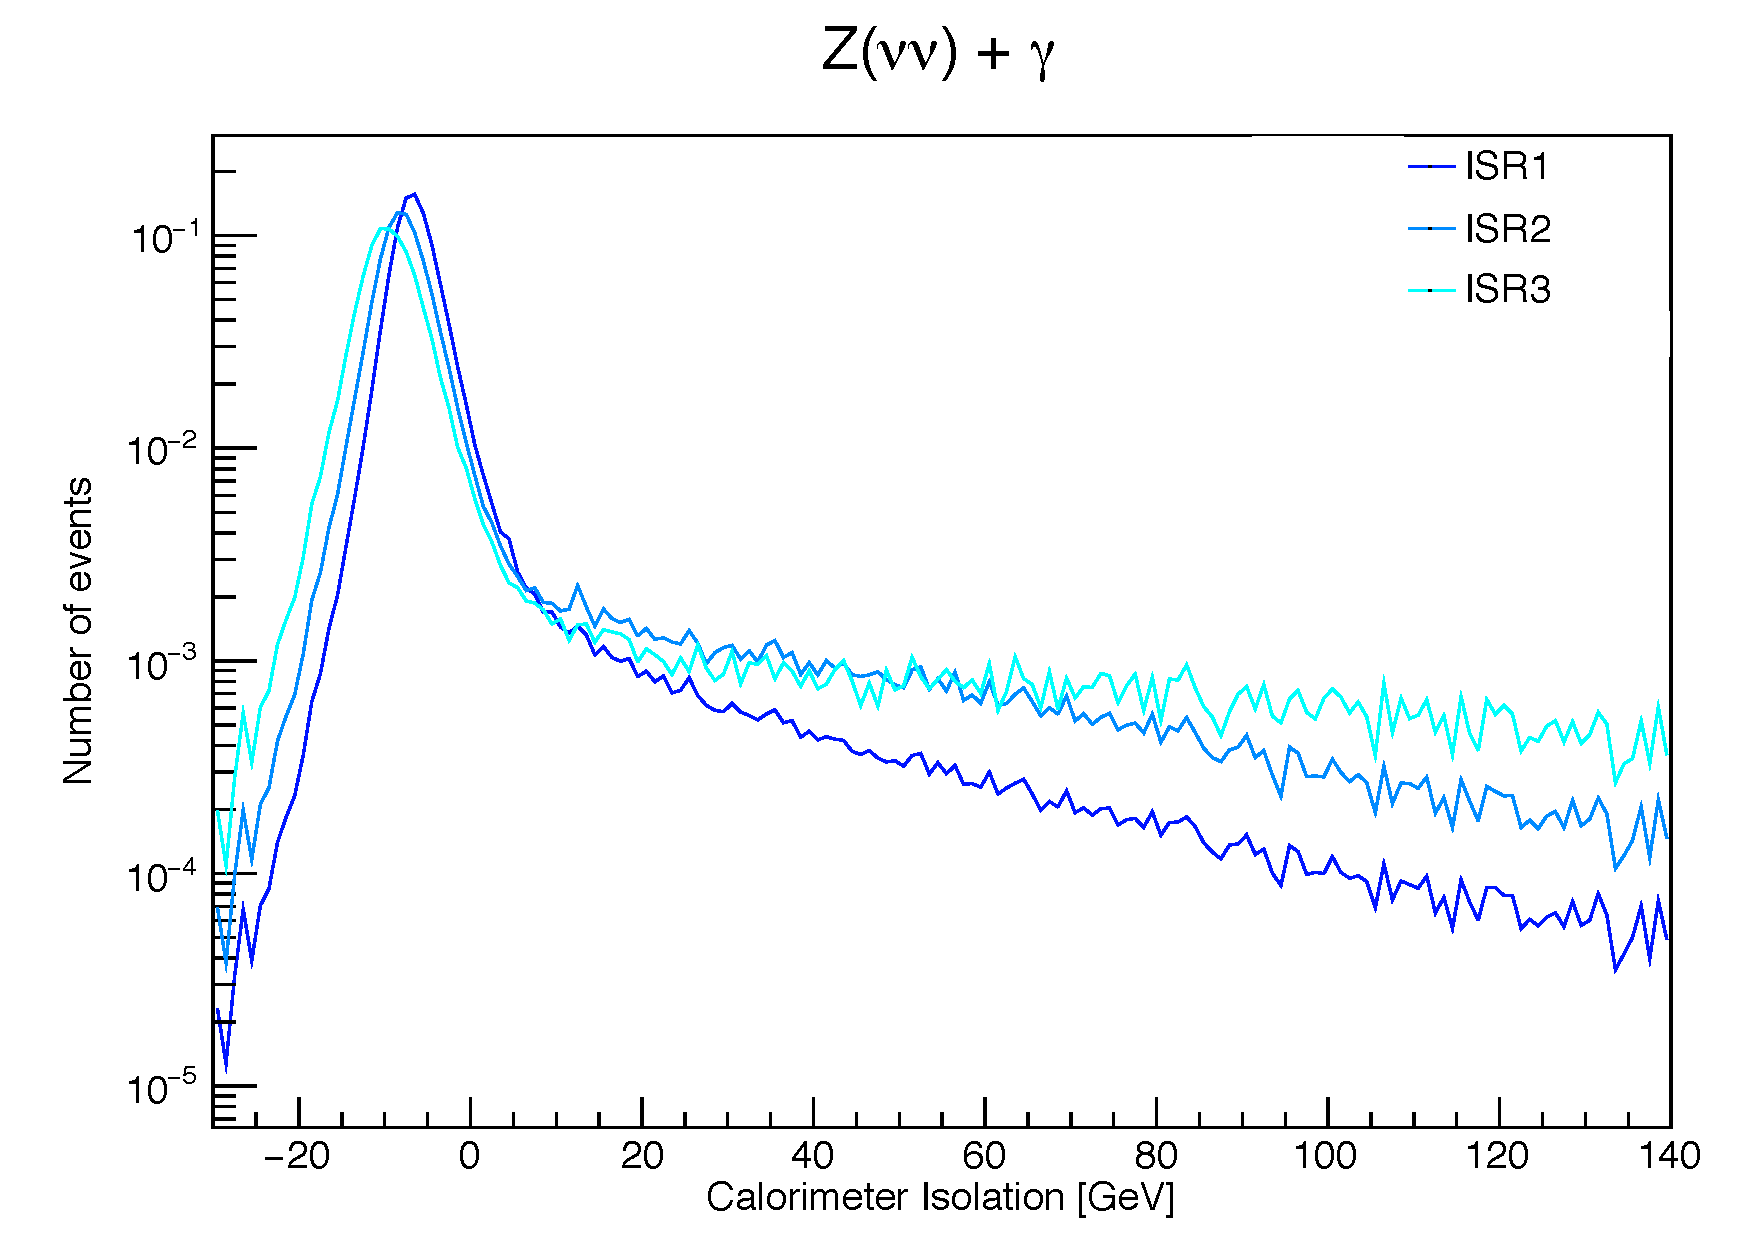
\includegraphics[width=10cm]{met_isolation_profiles.pdf}
    \caption{Normalized calorimetric isolation profiles, in logarithmic scale, of the Z($\nu \nu$) + $\gamma$ sample in the ISR1, ISR2 and ISR3.}
    \label{fig:met_isolation_profiles}
\end{figure}


\subsection{Correlation factor}

The correlation factors have been calculated separately on two background samples of Z + jets and W + jets. Results are reported in Fig. \ref{fig:R_MC}.


\begin{figure}[hbtp!]
    \centering
    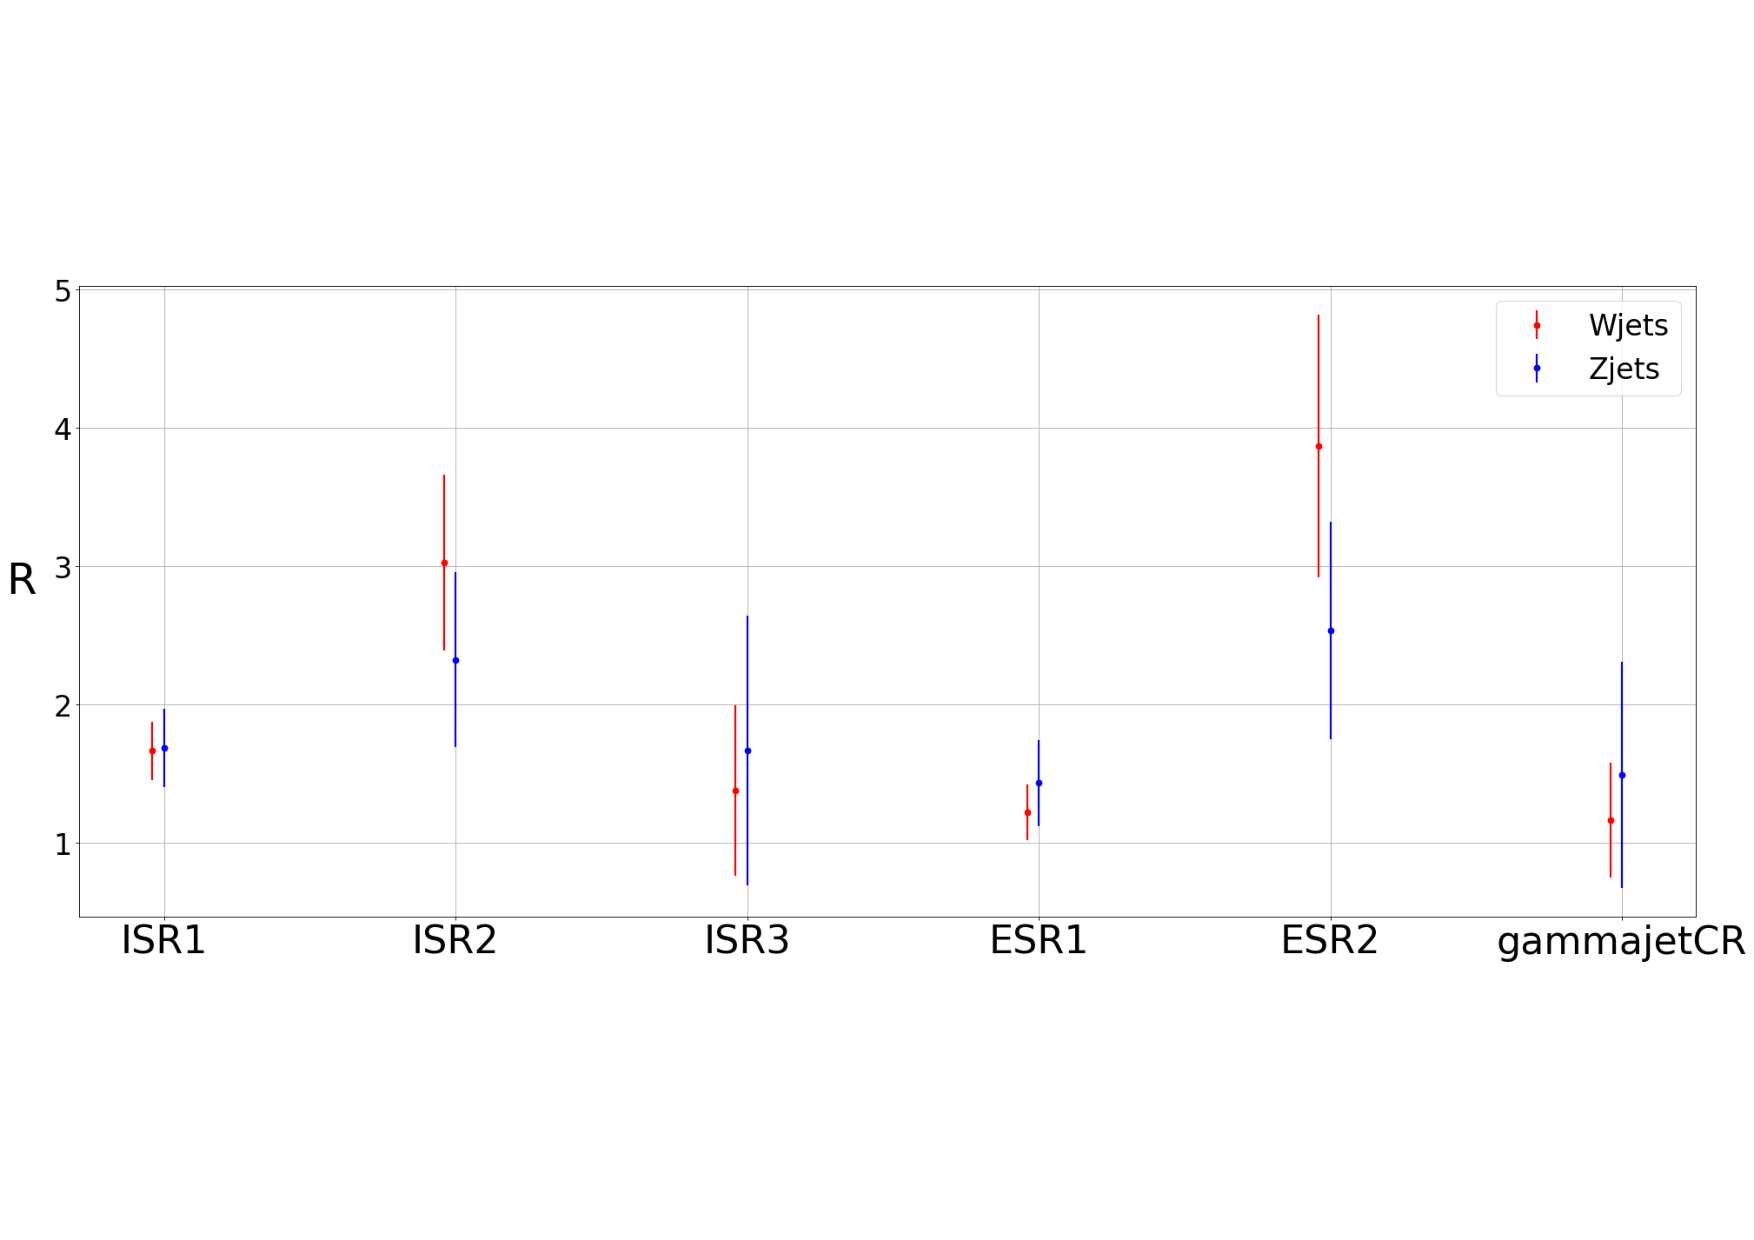
\includegraphics[width=12cm]{R_MC.pdf}
    \caption{Representation of the results obtained for the correlation factor using two samples of Z + jets and W + jets.}
    \label{fig:R_MC}
\end{figure}


As can be seen in the plot, the results are compatible within the uncertainties and don't show any evident systematics.



\subsection{R prime}

To evaluate the accuracy of the MC description of the correlation factor a special correlation factor ($R_{prime}$) in a completely not-isolated region has been computed: in this way it is possible to calculate it for both real data and MC without signal contamination problems. The MC used are the same as for the usual correlation factor, while data are the 2015-16 data. 
The populations in the not-isolated regions are divided by rectangular selections as Fig. \ref{fig:ABCD_prime} shows. The cuts on the track isolation and calorimetric isolation are chosen in order to maintain a good population in all these regions and are set to 0.2 and 50 GeV respectively, so that:

\begin{itemize}
    \item[-] $N^{A}_{prime}$: events with (3 GeV < calo isolation < 50 GeV and track isolation < 0.2) or (calo isolation < 3 GeV and 0.1 < track isolation < 0.2)
    \item[-] $N^{B}_{prime}$: events with (50 GeV < calo isolation < 100 GeV and track isolation < 1.0) or (calo isolation < 50 GeV and 0.2 < track isolation < 1.0)
\end{itemize}

and similarly for $M^{A}_{prime}$ and $M^{B}_{prime}$

\begin{figure}[hbtp!]
    \centering
    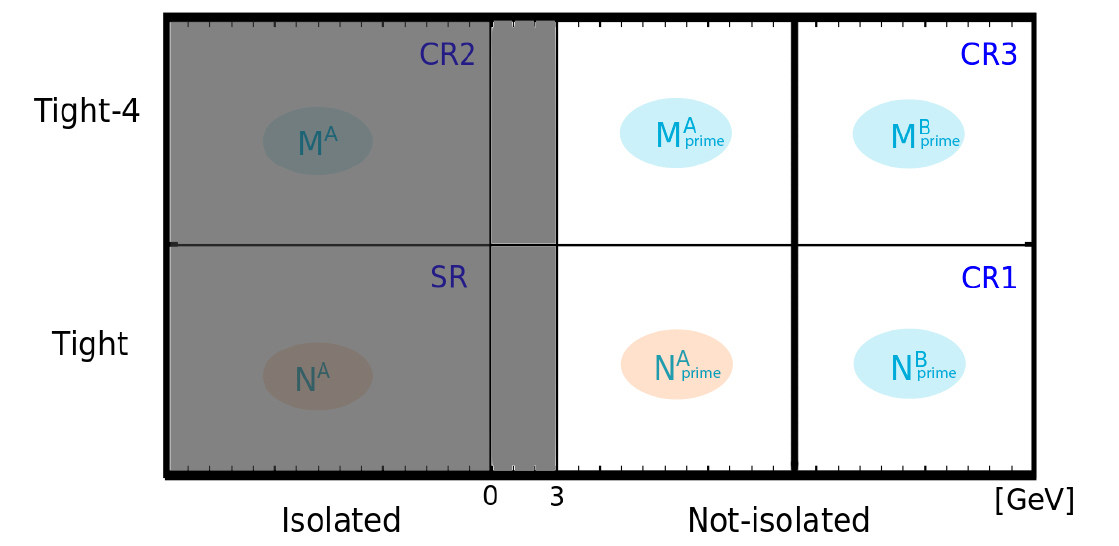
\includegraphics[width=10cm]{ABCD_prime.jpg}
    \caption{Scheme of the new regions defined to compute $R_{prime}$.}
    \label{fig:ABCD_prime}
\end{figure}


Results are reported in Fig. \ref{fig:R_prime}. The MC predictions for $R_{prime}$ and are compatible within uncertainties with those extracted from 2015-16 data, except in the gammajetCR where the statistics is very poor. Both data and MCs exhibits a $R_{prime}$ correlation factor close to 1.

\begin{figure}[hbtp!]
    \centering
    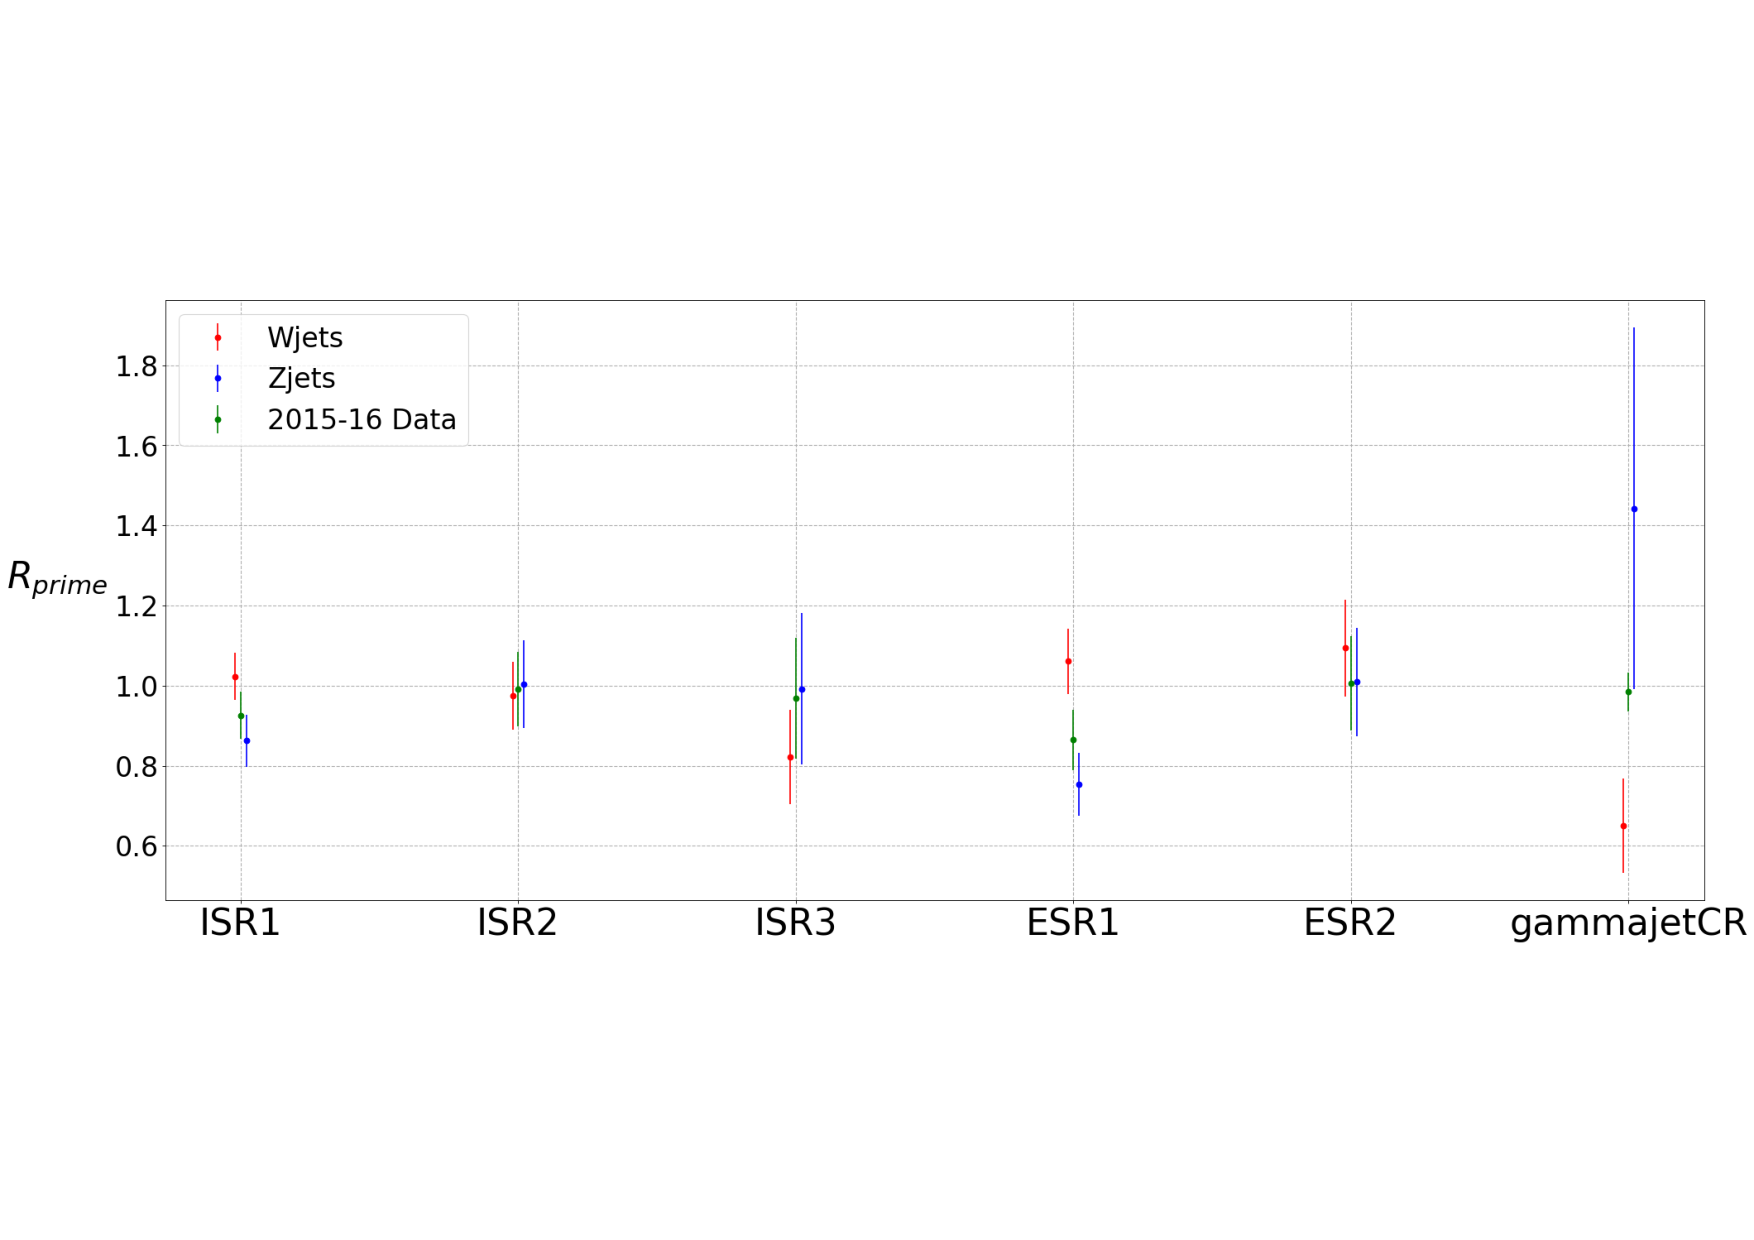
\includegraphics[width=12cm]{R_prime.pdf}
    \caption{Representation of the results obtained for $R_{prime}$ using two samples of Z + jets and W + jets.}
    \label{fig:R_prime}
\end{figure}


\subsection{Analysis} \label{coefficients_analysis}

For all the coefficients ($c_{1}$, $c_{2}$, $c_{3}$ and $R_{MC}$) a weighted mean over different MC samples is computed with its statistical uncertainties for the five SRs and the gammajetCR. Systematic uncertainties on $c_{1}$ and $c_{3}$ has been assigned as the RMS of the values from different MC. These uncertainties are propagated to the purity as the difference between the values obtained using $c_{x}$ varied up and down by the size of its uncertainty.

The 5+1 coefficients are applied to the 20+1 region of the analysis: each value is used in the corresponding SR and in all the Mono-Photon CRs (for example the results in the ISR1 will be used in the SR - ISR1, 1muCR - ISR1, 2muCR - ISR1 and 2eCR - ISR1) except for the coefficients in the gammajetCR that are treated only in this particular CR.


\section{Results}

It is now possible to compute the purities on 2015-16 data and compare them with the previous analysis results.

Statistical uncertainties are computed with the propagation of errors only from the real data populations, while the errors propagated from the coefficients are quoted as systematic errors as they are determined by the limited statistics of the MCs.

Systematic uncertainties on the purities, on the other hand, are obtained as discussed in Sec. \ref{Purity} and \ref{coefficients_analysis}. Having released the track isolation in CRs of the method, the gap between the isolated and not-isolated regions needs to be redefined. The now rectangular gap is varied respectively on the track isolation and calorimetric isolation as (0.05, 3 GeV) $\rightarrow$ (0.01, 2 GeV) or (0.05, 3 GeV) $\rightarrow$ (0.10, 4 GeV). The different systematic errors are finally summed in quadrature with the statistical errors propagated from the coefficients, giving the final systematic error on the purities. Finally the total error is the sum in quadrature of the total systematic and statistical errors.

Fig. \ref{fig:analysis_comparison} reports the results of fake photons numbers, both for the previous analysis and the published analysis \cite{Mono-Photon_article} on 2015-16 data, calculated as:

\begin{equation}
    N_{FakePhotons} = (1 - P) N^{A}
\end{equation}

where the errors are obtained simply by multiplying the error on $P$ by $N^{A}$. The two analysis results are compatible within uncertainties in each region of the analysis, although in the new analysis the systematic uncertainties are larger.

\begin{figure}[hbtp!]
    \centering
    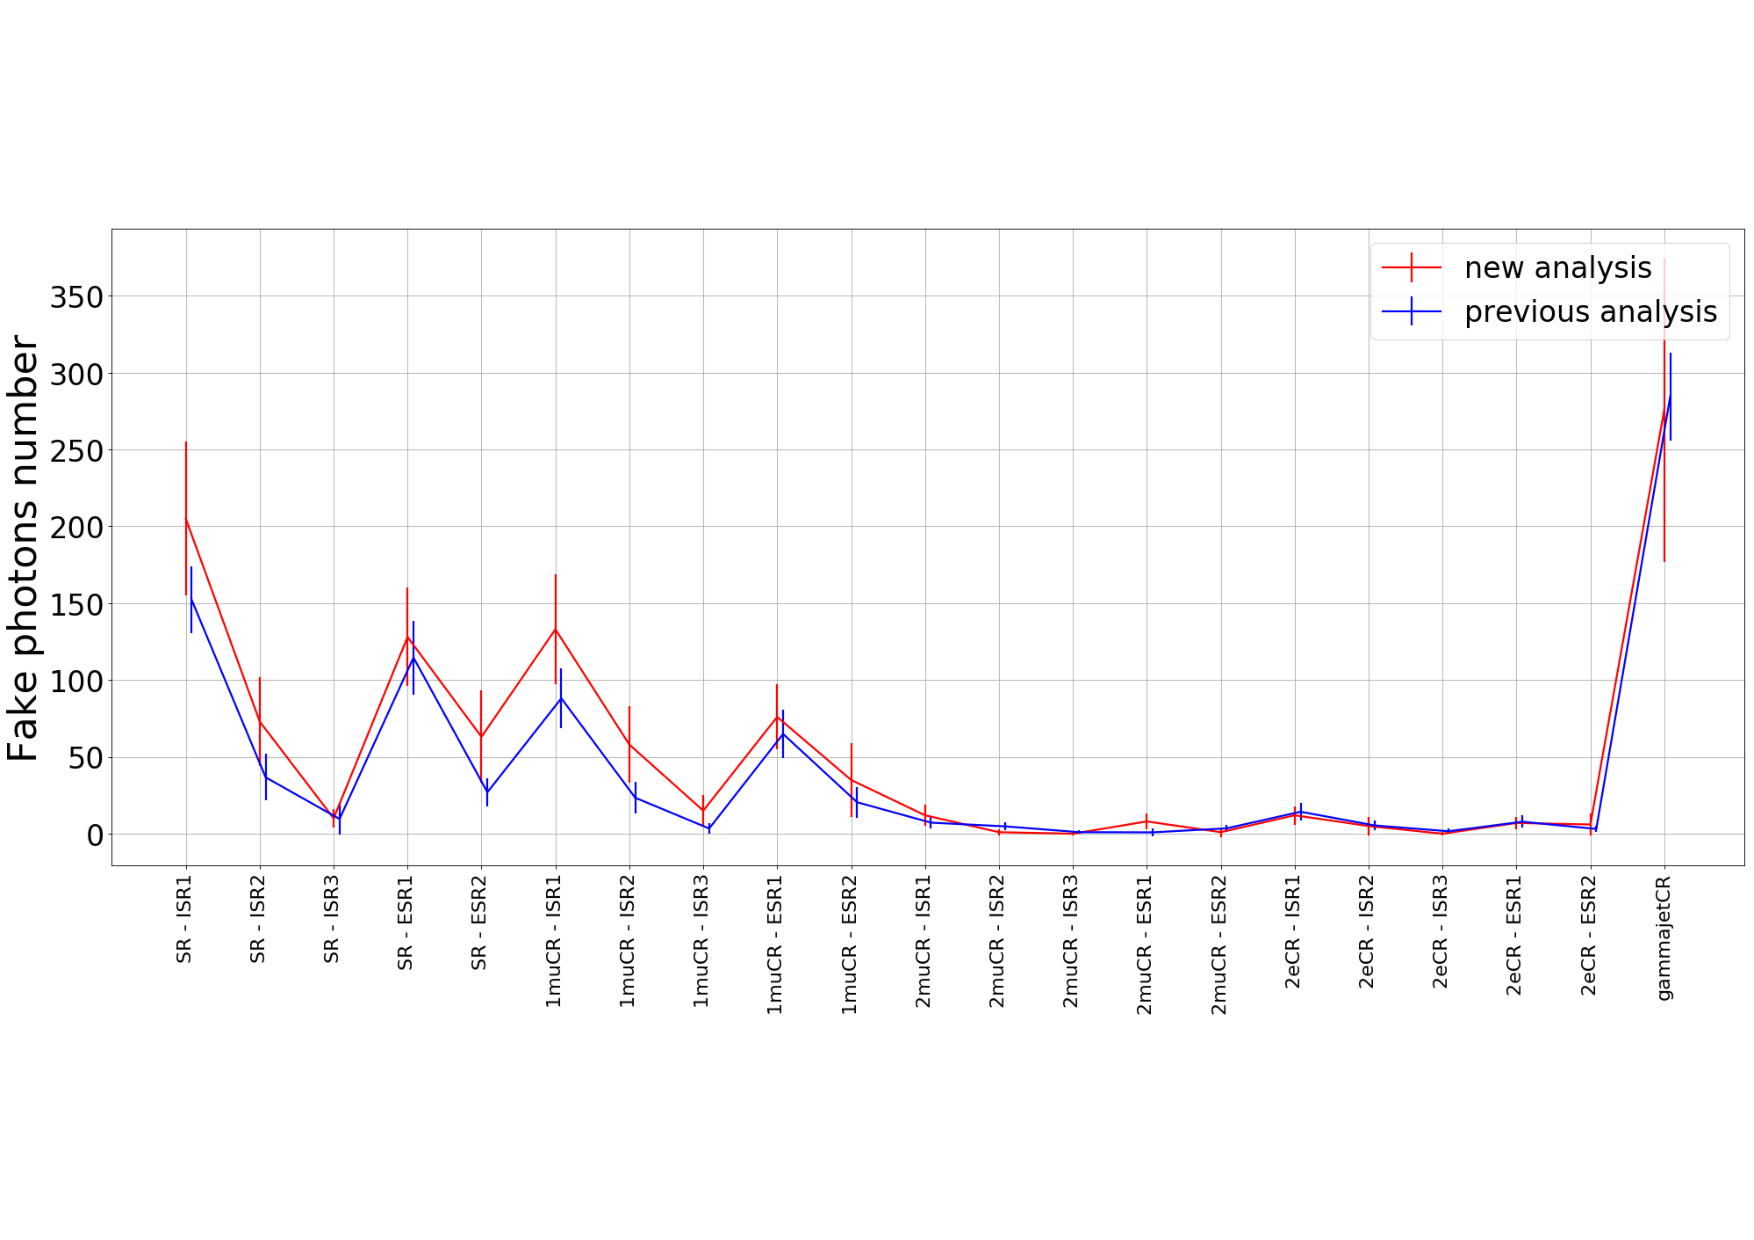
\includegraphics[width=12cm]{analysis_comparison.pdf}
    \caption{Comparison between results of the previous analysis (blu) and of the new analysis (red) on data taken during 2015-16.}
    \label{fig:analysis_comparison}
\end{figure}

Table \ref{tab:fake_photons} shows the details of the results obtained by the ongoing analysis on 2015-16 data. The results for the fake photons numbers in each region are dominated by the systematic error coming from the tightness control regions and by the statistical uncertainty on $R_{MC}$, while the uncertainties on the other coefficients don't really affect the total error.

\begin{table}[hbtp!]
\centering
\resizebox{\textwidth}{!}{%
\begin{tabular}{ccccccccccccc}
\hhline{=============} \\
regions & mean & stat. & \begin{tabular}[c]{@{}c@{}}tightness\\ syst.\end{tabular} & \begin{tabular}[c]{@{}c@{}}isolation\\ syst.\end{tabular} & \begin{tabular}[c]{@{}c@{}}c1\\ stat.\end{tabular} & \begin{tabular}[c]{@{}c@{}}c2\\ stat.\end{tabular} & \begin{tabular}[c]{@{}c@{}}c3\\ stat.\end{tabular} & \begin{tabular}[c]{@{}c@{}}R\\ stat.\end{tabular} & \begin{tabular}[c]{@{}c@{}}c1\\ syst.\end{tabular} & \begin{tabular}[c]{@{}c@{}}c3\\ syst.\end{tabular} & \begin{tabular}[c]{@{}c@{}}total\\ syst.\end{tabular} & \begin{tabular}[c]{@{}c@{}}total\\ error\end{tabular} \\ \hline \\
SR - ISR1 & 205 & 21 & 36 & 3 & 3 & 8 & 0 & 22 & 13 & 0 & 45 & 50 \\
SR - ISR2 & 73 & 15 & 19 & 2 & 2 & 6 & 0 & 13 & 6 & 0 & 25 & 29 \\
SR - ISR3 & 10 & 4 & 2 & 0 & 1 & 2 & 0 & 4 & 1 & 0 & 5 & 6 \\
SR - ESR1 & 128 & 15 & 20 & 5 & 2 & 6 & 0 & 17 & 7 & 0 & 29 & 32 \\
SR - ESR2 & 63 & 16 & 20 & 3 & 2 & 6 & 0 & 14 & 5 & 0 & 26 & 30 \\
1muCR - ISR1 & 133 & 15 & 28 & 5 & 1 & 3 & 0 & 14 & 4 & 0 & 32 & 36 \\
1muCR - ISR2 & 58 & 12 & 19 & 3 & 1 & 2 & 0 & 10 & 2 & 0 & 22 & 25 \\
1muCR - ISR3 & 15 & 5 & 6 & 1 & 0 & 1 & 0 & 6 & 0 & 0 & 8 & 10 \\
1muCR - ESR1 & 76 & 10 & 14 & 2 & 1 & 2 & 0 & 10 & 2 & 0 & 18 & 21 \\
1muCR - ESR2 & 35 & 9 & 21 & 1 & 1 & 2 & 0 & 7 & 2 & 0 & 22 & 24 \\
2muCR - ISR1 & 12 & 4 & 5 & 0 & 0 & 1 & 0 & 1 & 1 & 0 & 6 & 7 \\
2muCR - ISR2 & 1 & 2 & 1 & 0 & 0 & 1 & 0 & 0 & 0 & 0 & 1 & 2 \\
2muCR - ISR3 & -0 & 0 & 0 & 0 & 0 & 0 & 0 & 0 & 0 & 0 & 0 & 1 \\
2muCR - ESR1 & 8 & 3 & 3 & 1 & 0 & 0 & 0 & 1 & 1 & 0 & 4 & 5 \\
2muCR - ESR2 & 1 & 3 & 1 & 0 & 0 & 1 & 0 & 0 & 0 & 0 & 1 & 3 \\
2eCR - ISR1 & 12 & 5 & 3 & 1 & 0 & 0 & 0 & 1 & 1 & 0 & 4 & 6 \\
2eCR - ISR2 & 5 & 4 & 4 & 0 & 0 & 0 & 0 & 1 & 0 & 0 & 4 & 6 \\
2eCR - ISR3 & 0 & 1 & 0 & 0 & 0 & 0 & 0 & 0 & 0 & 0 & 0 & 1 \\
2eCR - ESR1 & 7 & 3 & 3 & 0 & 0 & 0 & 0 & 1 & 1 & 0 & 3 & 4 \\
2eCR - ESR2 & 6 & 5 & 5 & 1 & 0 & 0 & 0 & 1 & 0 & 0 & 5 & 7 \\
gammajetCR & 276 & 18 & 26 & 20 & 8 & 32 & 1 & 85 & 5 & 0 & 97 & 99 \\ \hhline{=============}
\end{tabular}%
}
\caption{Results for fake photon numbers of the current analysis of 2015-16 data with statistical (stat.) and systematic (syst.) errors.}
\label{tab:fake_photons}
\end{table}


\end{document}
